\section{Practical Implementation Plan}

This section outlines the specific implementation plan for the thesis project,
detailing the project structure, work patterns and the benefits of this approach.

The current project structure is designed into 9 major folders,
each with a specific storage function as briefly described in
Table \textcolor{blue}{\ref{tab:project_structure}}.

\begin{table}[!h]
\centering
\caption{Project folder structure and description}
\label{tab:project_structure}
\renewcommand{\arraystretch}{1.3}
\begin{tabular}{p{3cm}p{10cm}}
\hline
\textbf{Folder} & \textbf{Description} \\
\hline
\texttt{src/} & Core source code package (\texttt{ecoindex}) with reusable analysis modules. \\
\texttt{notebooks/} & Interactive Jupyter notebooks for prototyping and exploratory work that majorly achieves by modules from \textit{src}. \\
\texttt{tests/} & Unit tests for packages wrote in \texttt{ecoindex}, using \texttt{pytest} to ensure correctness and reliability. \\
\texttt{configs/} & Centralized configuration (random seeds, parameters, file paths),
collective containers for important parameters. \\
\texttt{data/} & Raw and processed datasets, organized for reproducibility. \\
\texttt{artifacts/} & Outputs not easily reproducible, e.g., trained models or serialized results. \\
\texttt{figures/} & Generated plots, charts, and visualizations for reporting. \\
\texttt{reference/} & External references, guidelines, and supporting documentation. \\
\texttt{documents/} & Thesis drafts, LaTeX files, lying close to results folders to keep
synchronous with the results.\\
\hline
\end{tabular}
\end{table}

The following two subsections will elaborate on the principles and rationales behind this project structure design,
and use a specific example to demonstrate the codebase design and working pattern.

\subsection{Research Professional Codebases}
To make a good research professional codebase, I want to follow the principles of modularity, reusability and maintainability.
This means organizing code into reusable components, documenting functionality clearly, 
doing tests for all components, and ensuring that the codebase can be easily understood and modified.

Out of these principles, the code structure and organization become paramount in achieving the work.
It has to be admitted that such structure would cost more time in setting up and analysing 
the meta data, significant amount of time when compared to directly writing the code in a single 
file. However, with the progress of the project, the benefits of this structure will become apparent
and obviously accelerate the research process, which is visible and achievable to
a non-computer science student with the support of these Generative AI tools.

The following example shows a quick starting point for the codebase, where I wrote
and wrote some functions to achieve a given data transformation operation, wrapping
it in a clear structured way into original data frame and testing the correctness 
of these operations. 

\subsubsection{Modularized Function implementation and lightweight application}

As it was mentioned in the methodology part, I wanted to continuously add computed 
results, which were sitewise specific, into the original data frame meanwhile
keeping the whole data frame tiny and efficient. Assuming I had the three raw data sets in my
\textit{data/raw} folder, and I wanted to do a hellinger transformation on the
taxa data set and export the transformed data into the \textit{data/processed} folder.
To achieve this complete operation, I would need the following modules and functions within them:

\begin{table}[!h]
\centering
\caption{Temporary Code Structure for Hellinger Transformation and Integrity of Data Frame}
\label{tab:module_structure}
\renewcommand{\arraystretch}{1.3}
\begin{tabular}{p{3.5cm}p{9.5cm}}
\hline
\textbf{Module} & \textbf{Description} \\
\hline
\textit{src/config.py} & Configuration management for centralized parameter storage and project settings,
like file paths and processing options. \\
\hline
\textit{src/cleaning.py} & Data cleaning utilities for handling missing values, outliers, and data quality issues. \\
\hline
\textit{src/ingest.py} & Data ingestion functions for loading raw datasets from various sources and formats. \\
\hline
% \textit{src/data-io.py} & Input/output operations for reading and writing data files in different formats. \\
% \hline
\textit{src/dataframe-ops.py} & DataFrame manipulation utilities for wrapping new information into layered data frames \\
\hline
\textit{src/transform.py} & Data transformation functions including ecological transformations like Hellinger. \\
\hline
\textit{src/pipeline.py} & Pipeline orchestration for chaining multiple data processing steps together. \\
\hline
\textit{notebooks/0-interim-data.py} & Notebook to invoke the above functions in practical scenarios,
lightweight code snippets for quick testing and validation. \\
\hline
\textit{tests/test-*.py} & Unit tests for validating the functionality of individual modules and functions
in above modules(\textit{src/*}). \\
\hline
\end{tabular}
\end{table}

The whole modules are not only designed for Hellinger Transformation, but it is a good example and there will be more
functions and module added in this structure to make the project concise and reproducible.

\begin{figure}[!h]
    \centering
    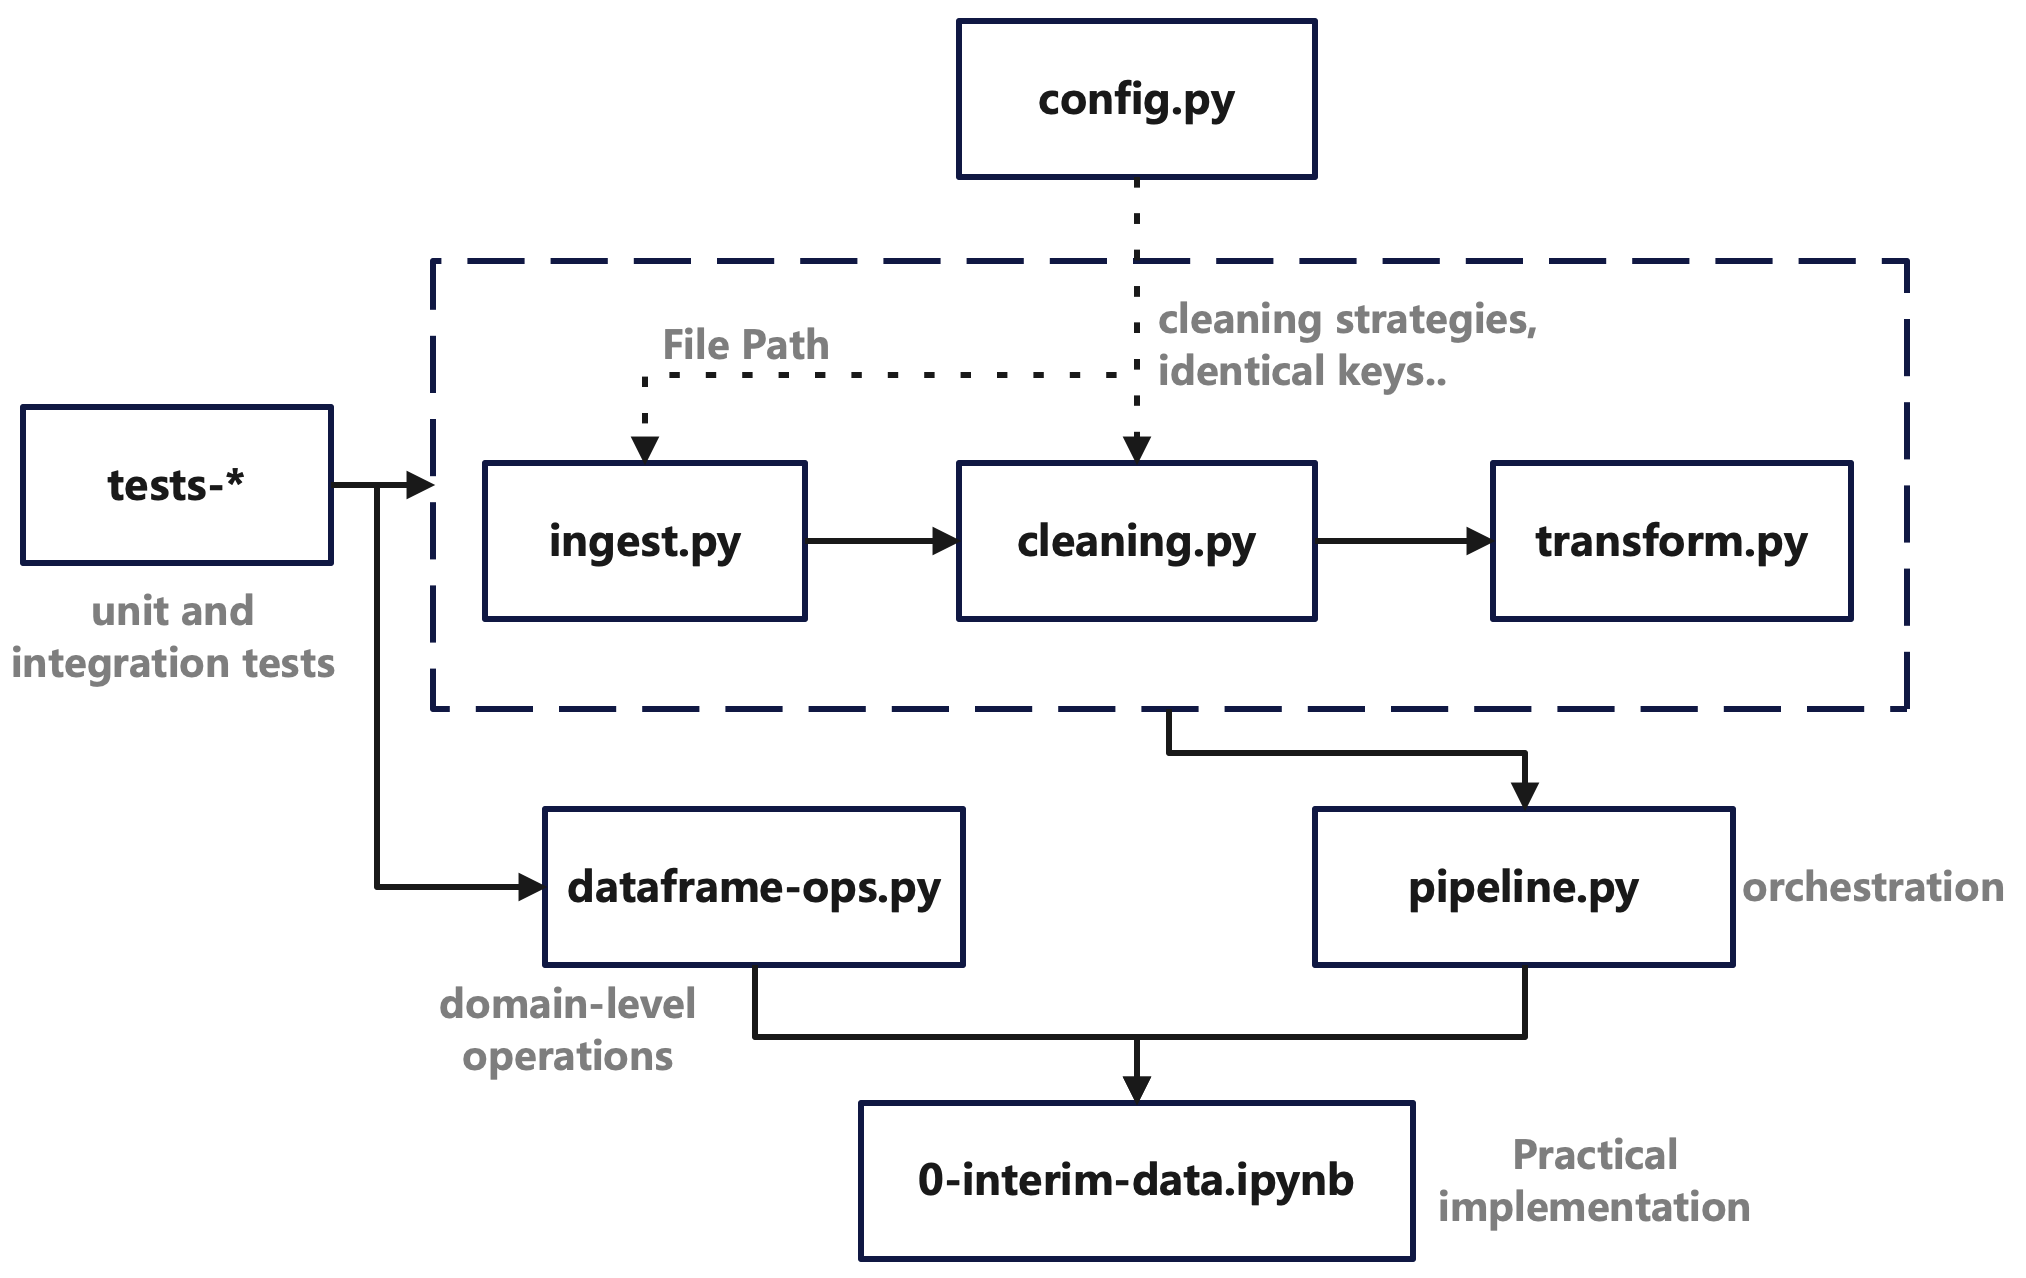
\includegraphics[width=0.9\textwidth]{../results/preliminary_results/implementPlan_example_codebase.png}
    \caption{Demonstration of Workflow for Implementing and Integrating Hellinger Transformation into Complete Data Processing Pipeline}
    \label{fig:implementPlan_example_codebase}
\end{figure}

With this highly integrated modularization, the previously long and complex code can be enclosed in these
separated modules and the application work can be achieved by a few lines of code.
Like the following lines of code in Figure \textcolor{blue}{\ref{fig:example_lightweight_code_completed}} achieve the whole transformation and data merging work
in the Jupyter notebook, which used to require much more extensive and vulnerable code within the same notebook:

\begin{figure}[!h]
    \centering
    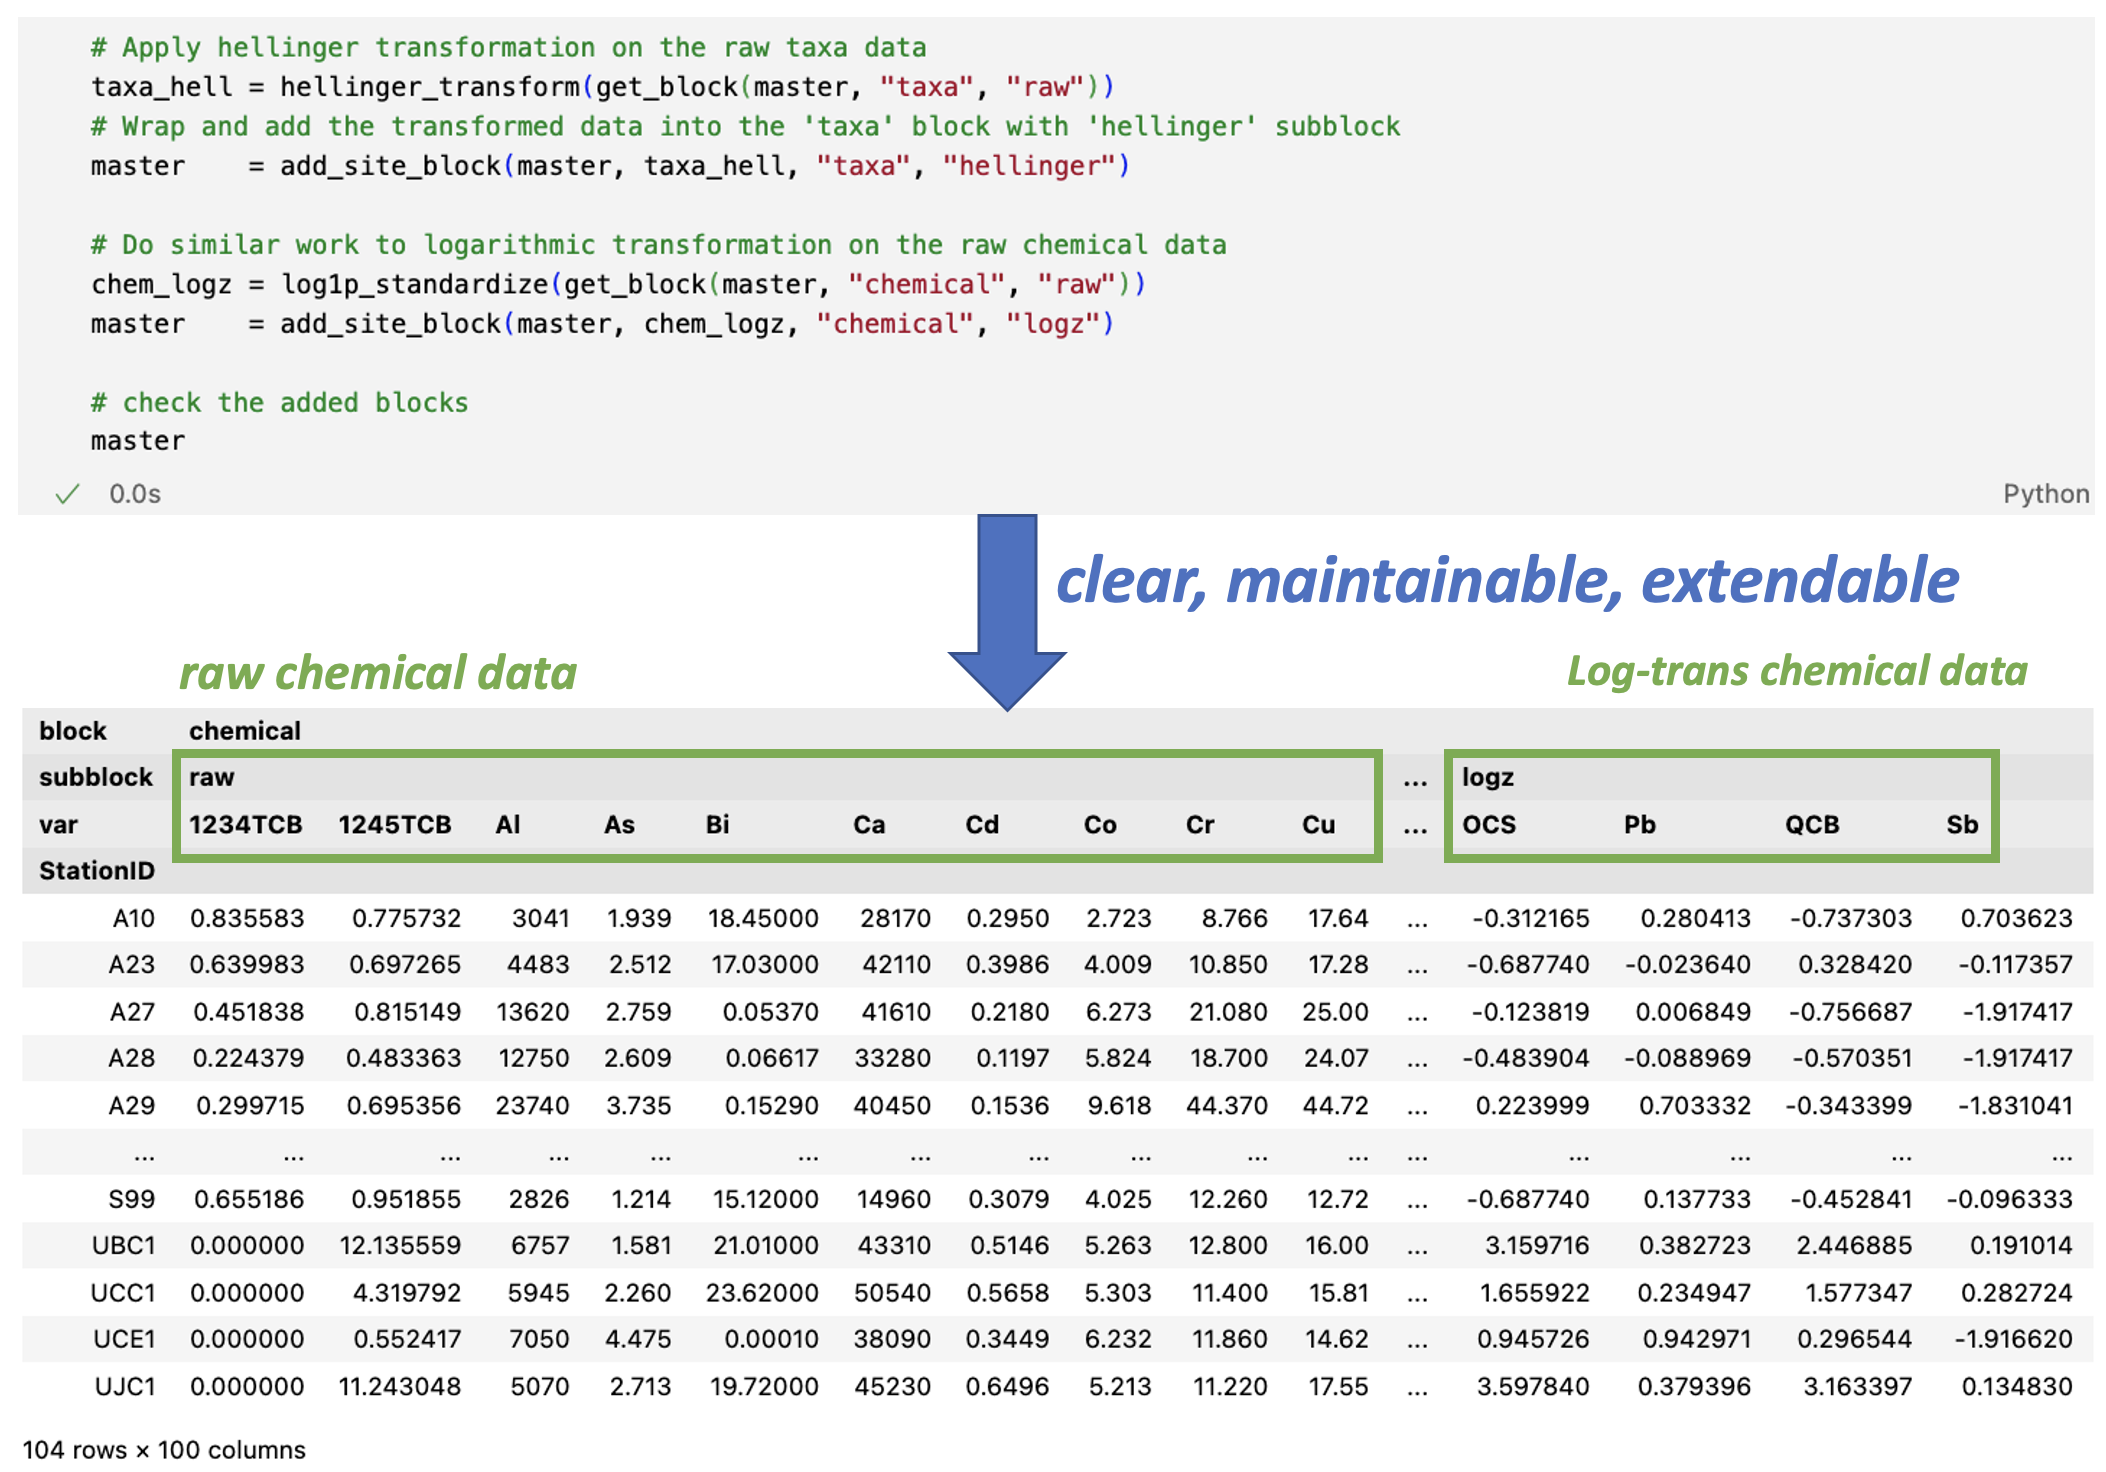
\includegraphics[width=0.9\textwidth]{../results/preliminary_results/example_lightweight_code_completed.png}
    \caption{The lines of code needed to achieve the above discussed operations in practical scenarios and the resulting integrated data frame from the operation}
    \label{fig:example_lightweight_code_completed}
\end{figure}




\subsection{General Project Structure and Rationale}

Generally speaking, the project follows a modular and well-organized structure to support both 
research reproducibility and software engineering best practices.
The folder layout is as follows:

\begin{itemize}
    \item \textbf{configs}: centralizes configuration files (e.g., paths, random seeds, parameter settings), ensuring experiments are reproducible and adjustable without modifying code.
    \item \textbf{data}: stores raw, interim, and processed datasets in a structured hierarchy, making data provenance transparent and simplifying pipeline automation.
    \item \textbf{documents}: contains draft texts, LaTeX notes, and thesis-related writeups, providing a bridge between research outputs and manuscript preparation.
    \item \textbf{figures}: keeps all generated visualizations, plots, and diagrams organized for easy reuse in the thesis and publications.
    \item \textbf{notebooks}: hosts exploratory Jupyter notebooks, which serve as an interface for practical implementation, quick testing, and visualization.
    \item \textbf{reference}: used for bibliographic resources, papers, and supplementary literature, ensuring traceability of scientific background.
    \item \textbf{src}: holds the main source code in a modular format (e.g., \texttt{ingest.py}, \texttt{cleaning.py}, \texttt{pipeline.py}), which separates concerns between ingestion, cleaning, transformation, and higher-level operations.
    \item \textbf{tests}: includes unit tests and validation scripts to ensure correctness and robustness of each module across different scenarios.
    \item \textbf{artifacts}: stores intermediate results, logs, and model checkpoints, preserving computational outcomes for reproducibility and debugging.
    \item \textbf{pyproject.toml}: defines the project environment, dependencies, and metadata, which standardizes reproducibility across systems.
\end{itemize}

\noindent This design provides several benefits:
\begin{enumerate}
    \item \textbf{Reproducibility}: Configurations, raw data, and processed results are explicitly separated, making workflows transparent and repeatable.
    \item \textbf{Scalability}: Modular code in \texttt{src/} and standardized data storage enable extensions (e.g., adding new datasets or models) with minimal disruption.
    \item \textbf{Clarity}: Clear distinction between code, data, results, and documentation reduces confusion and facilitates collaboration or future reuse.
    \item \textbf{Professionalism}: The structure aligns with common practices in industrial data science and academic research, ensuring maintainability and credibility of the project.
\end{enumerate}

